\documentclass[12pt]{article}
\usepackage[margin=1in]{geometry}
\usepackage{amsmath}
\usepackage{amssymb}
\usepackage{amsthm}
\usepackage{amsfonts}
\usepackage{graphicx}

\theoremstyle{definition}
\newtheorem{theorem}{Theorem}[section]
\newtheorem{lemma}[theorem]{Lemma}
\newtheorem{corollary}[theorem]{Corollary}
\newtheorem{definition}[theorem]{Definition}
\newtheorem{proposition}[theorem]{Proposition}

\title{Finiteness of Class Groups and the Minkowski Theorem}
\author{}
\date{}

\begin{document}

\maketitle

\begin{abstract}
This paper develops the algebraic number theory and geometry of numbers needed to prove the finiteness of 
ideal class groups of number fields. It introduces the basic language of algebraic integers, Dedekind domains, ideals, 
norms, and discriminants, then turns to lattices and the Minkowski embedding to connect number theory with geometry. 
Using Minkowski's lattice point theorem, the paper derives bounds on the norms of ideals representing ideal classes and 
concludes that the class group of a number field is finite. 
\end{abstract}


\section{Introduction}
\label{sec:intro}
% Motivation and historical context



\section{Algebraic Number Theory Preliminaries}
\label{sec:preliminaries}
To get started we need a few basic number theory definitions and notations explained. 
\begin{definition}
    An \textbf{algebraic number field} is a finite $\mathbb{Q}$-extension field, $K$, such that every element in K is the root of some polynomial with rational coefficients. 
\end{definition}
A simple example of an algebraic number field is $\mathbb{Q}(\sqrt{5})$ because every element, $x=a+b\sqrt{5}$, $a,b \in \mathbb{Q}$ is a root of some polynomial in $\mathbb{Q}[x]$:
\[x=a+b\sqrt{5} \implies x-a=b\sqrt{5} \implies x^2 - 2ax + a^2 - 5b^2 = 0 \]
\begin{definition}
    Let $R \subseteq S$ be commutative rings. $s \in S$ is \textbf{integral} over $R$ if s is a root of a monic
    polynomial $f(x)\in R[x]$. $S$ is integral over $R$ if all $s \in S$ are integral over $R$.
\end{definition}
Take for example $i \in \mathbb{C}$. $i$ is the root of $x^2+1$ which is a monic polynomial with integer coefficients. So $i$ is integral over $\mathbb{Z}$.
However, look at $\frac{1}{2} \in \mathbb{Q}$. $\frac{1}{2}$ is a root of the polynomials $2x-1 = 0 $ and $x-\frac{1}{2} = 0$ neither of which are both monic and have integer coefficients. 
So, $\frac{1}{2}$ is not integral over $\mathbb{Z}$. 
\begin{definition}
    Let $R \subseteq S$ be commutative rings. The \textbf{integral closure} of $R$ in $S$ is the set of all elements in $S$ that are integral over $R$:
    \[\bar{R} = \{s \in S | s \text{ integral over } R \} \]
    $R$ is \textbf{integrally closed} in $S$ if $\bar{R}=R$.
\end{definition}
Let's look at the integral closure of $R=\mathbb{Z}$ in the field $S=\mathbb{Q}(\sqrt{5})$.
For sure $\mathbb{Z}[\sqrt{5}]$ is in the integral closure. As we saw above,
\[
x=a+b\sqrt{5} \implies x^2 - 2ax + a^2 - 5b^2 = 0
\]
But in this case, $a,b \in \mathbb{Z}$ so the above polynomial is monic and in $\mathbb{Z}[x]$.
However, $\frac{1+\sqrt{5}}{2}$ is also in the integral closure:
\[
x=\frac{1+\sqrt{5}}{2} \implies 2x - 1 = \sqrt{5} \implies 4x^2 -4x + 1 = 5 \implies x^2 - x - 1 = 0
\]
So, the integral closure of $\mathbb{Z}$ in $\mathbb{Q}(\sqrt{5})$ is actually $\mathbb{Z}[\frac{1+\sqrt{5}}{2}]$.

This brings us to rings of algebraic integers. 

\begin{definition}
    All elements in an algebraic number field, $K$, that are roots of monic polynomials with integer coefficients form a ring called the \textbf{ring of algebraic integers: $\mathcal{O}_K$} or a \textbf{number ring}.
\end{definition}

In other words, $\mathcal{O}_K$ is the integral closure of $\mathbb{Z}$ in $K$. $\mathcal{O}_K$ is the set of all elements in $K$ that may not look like integers but they "act" like integers. 
The standard integers $\mathbb{Z}$ form a ring; you can only leave $\mathbb{Z}$ by dividing. $\mathcal{O}_K$ behaves the same way and as we'll see later, ideals in $\mathcal{O}_K$ also factor uniquely into prime ideals, similar
to how integers factor uniquely into prime numbers. 
So, to keep using our $\mathbb{Q}(\sqrt{5})$ example, the ring of algebraic integers for $K = \mathbb{Q}(\sqrt{5})$ is $\mathbb{Z}[\frac{1+\sqrt{5}}{2}]$.

\begin{definition}
    Let $K$ be a number field of degree $n$ over $\mathbb{Q}$. Let $\sigma_1, \sigma_2, ..., \sigma_n$ denote the
    $n$ embeddings of $K$ in $\mathbb{C}$ that fix $\mathbb{Q}$. The \textbf{discriminant} of the set $\{\theta_1, \theta_2, ..., \theta_n\}$, denoted
    disc$(\theta_1, \theta_2, ..., \theta_n)$, is defined absolute
    \[\text{disc}(\theta_1, \theta_2, ..., \theta_n) = \det[\sigma_j(\theta_i)]^2 = 
    \det\begin{bmatrix} \sigma_1(\theta_1) & \sigma_2(\theta_1) & ... & \sigma_n(\theta_1) \\ \sigma_1(\theta_2) & \sigma_2(\theta_2) & ... & \sigma_n(\theta_2) \\ ... & ... & ... & ... \\ \sigma_1(\theta_n) & \sigma_2(\theta_n) & ... & \sigma_n(\theta_n) \end{bmatrix}^2\]
\end{definition}

When referring to the discriminant of a basis of $\mathcal{O}_K$ as opposed to the discriminant of an element(s), the discriminant is referred to absolute
the \textbf{field discriminant} of $K$ and denoted $d(K)$. Furthermore the discriminant is independent of the choice of integral basis. The discriminant gives us important
information about how ideals factor in the number ring. It also can be used as a tool to verify if a set of elements form an integral basis for $\mathcal{O}_K$. 

While every number ring is an integral domain, it's generally not a unique factorization domain. However, it has its own unique structure; 
every number ring is what's known as a Dedekind Domain. 

\begin{definition}
    An integral domain, $R$, is called a \textbf{Dedekind Domain} when
    \begin{enumerate}
        \item[(i)] Every ideal of $R$ is finitely generated
        \item[(ii)] Every non-zero prime ideal is maximal
        \item[(iii)] $R$ is integrally closed in its field of fractions
        \[ K = \{ \frac{\alpha}{\beta} | \alpha, \beta \in R, \beta \neq 0 \}\]
        i.e. the only elemets $\frac{\alpha}{\beta}\in K$ that are integral over $R$ are $\frac{\alpha}{\beta}\in R$.
    \end{enumerate}
\end{definition}

This allows us to be able to factor every ideal in a number ring into a product of prime ideals which will be useful later. 

\begin{theorem}
    In a Dedekind domain, every ideal contains a product of prime ideals. 
\end{theorem}

\begin{definition}
    Let $\mathcal{O}$ be a Dedekind Domain and $K$ is its field of fractions. A \textbf{fractional ideal} of $K$ is a set of the form $\alpha I, \alpha \in K, \alpha \neq 0$, where $I$ is a non-zero ideal of $\mathcal{O}$.
\end{definition}

\begin{definition}
    An \textbf{integral ideal} in a ring $R$ is an additive subgroup $I \subset R$ such that $ra \in I, \forall r\in R, a \in I$.
    An \textbf{integral ideal} can also be obtained by multiplying a fractional ideal, by a common denominator such that it is back in $R$.
\end{definition}

\begin{definition}
    A \textbf{factor group} is formed by dividing out a group $R$ by another group $I$ and is denoted $R/I$.
    The elements of $R/I$ can be regarded as equivalence classes for the congruence relation on $R$ defined by
    \[ a \equiv b \pmod I \iff a-b \in I \]
\end{definition}

\begin{definition}
    The \textbf{order} of some factor group $G/H$ is the number of elements in $G/H$. Equivalently, it is 
    the number of cosets of $H$ in $G$ otherwise known as the \textbf{index}: $(G:H)$.
\end{definition}

\begin{definition}
    Let $K$ be an algebraic number field. Let $J_K$ be the group of non-zero fractional and integral ideals of $\mathcal{O}_K$.
    Let $P_K$ be the subgroup of principal ideals of $J_K$. The \textbf{ideal class group} of $K$ is denoted $Cl_K$ and is the factor group of $J_K/P_K$.
\end{definition}

\begin{definition}
    The order of the ideal class group of $K$, denoted $h_K$ is called the \textbf{class number} of K.
\end{definition}

\begin{theorem}
    Let $K$ be an algebraic number field. Then\\
    $h_K = 1 \iff \mathcal{O}_K$ is a principal ideal domain $\iff \mathcal{O}_K$ is a unique factorizatin domain. 
\end{theorem}

\begin{definition}
    Let ${v_1, v_2, ..., v_m}$ be a set of $m$ linearly independent vectors in $\mathbb{R}^n$, a \textbf{lattice} $\Gamma$ is the set of all integer linear combinations of those basis vectors:
    \[\Gamma = \{\sum_{i=1}^{m}a_iv_i | a_i \in \mathbb{Z} \}\]
    The elements of $\Gamma$ are called \textbf{lattice points}. The lattice is called \textbf{complete} if $m=n$. The \textbf{volume} of the \textbf{funadmental mesh} of $\Gamma$ is
    \[vol(\Gamma) = |\det(A)| \]
    where $$A = \begin{bmatrix} | & | & & | \\ v_1 & v_2 & \dots & v_m \\ | & | & & | \end{bmatrix}$$
\end{definition}
A simple example of a lattice is the standard integer lattice $\mathbb{Z}^2$, which forms a grid of all integer pairs in 2D space. In this case $m=2$ so the lattice is complete and we use the standard basis
$v_1=(1,0)$ and $v_2=(0,1)$. See Figure \ref{fig:z2lattice} for a visual. The volume of the fundamental mesh of $\mathbb{Z}^2$ is simple to calculate:
\[vol(\mathbb{Z}^2) = |\det(\begin{bmatrix} 1 & 0 \\ 0 & 1 \end{bmatrix})| = |1-0| = 1\]
\begin{figure}[h]
    \centering
    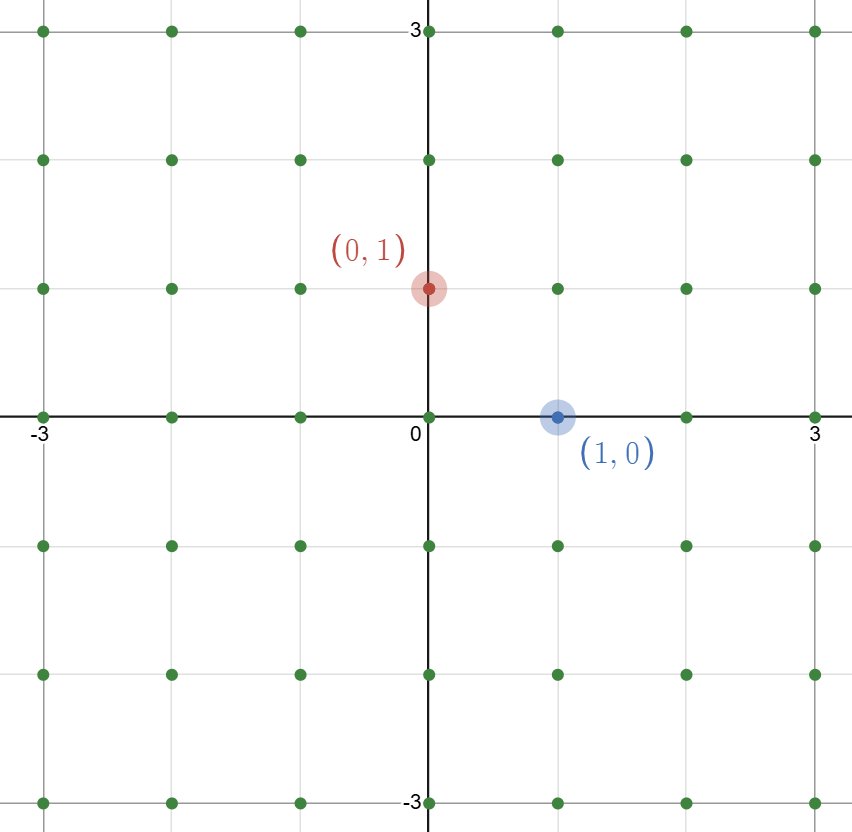
\includegraphics[width=0.5\textwidth]{figures/Z^2Lattice.png}
    \caption{The $\mathbb{Z}^2$ lattice in 2D space}
    \label{fig:z2lattice}
\end{figure}

\begin{definition}
    A subset $S$ of $\mathbb{R}^n$ is said to \textbf{convex} if 
    \[t\beta + (1-t)\gamma \in S \quad \forall \beta, \gamma \in S \text{ and } \forall t \in \mathbb{R}\]
\end{definition}

Visually, we can think of a set of points as a shape that is convex when a line connecting 2 points in the shape is also entirely in the shape. 
For example, a circle, square or ellipse is convex but a star or crescent moon is not. You could draw a line between 2 points on either "arm" of the
star and the line would pass outside of the shape. 

\begin{definition}
    A subset $S$ of $\mathbb{R}^n$ is said to be \textbf{centrally symmetric} if 
    \[-\alpha \in S \quad \forall \alpha \in S\]
\end{definition}

In other words, a shape is centrally symmetric if it looks exactly the same when rotated 180\textdegree around the origin.

\begin{theorem}{(Minkowski's Lattice Point Theorem).} 
    Let $\Gamma$ be a complete lattice in $\mathbb{R}^n$, and let $X$ be a centrally symmetric,
    convex subset of $\mathbb{R}^n$. Suppose that 
    \[vol(X) > 2^nvol(\Gamma).\]
    Then $X$ contains at least one nonzero lattice point $\gamma \in \Gamma$.
\end{theorem}

\begin{definition}
    Let $K/\mathbb{Q}$ be a finite extension, and let $I \neq 0$ be an ideal of $\mathcal{O}_K$. The \textbf{absolute norm} of $I$ is given by
    \[ \mathfrak{N}(I) = (\mathcal{O}_K : I)\]
\end{definition}

\begin{definition}
    Let $K$ be a number field of degree $n = r + 2s$, with $r$ real embeddings $\rho_1, \dots, \rho_r$ and $s$ pairs of complex conjugate embeddings $\sigma_1, \bar{\sigma}_1, \dots, \sigma_s, \bar{\sigma}_s$. The \textbf{canonical embedding} (or Minkowski embedding) is the injective ring homomorphism $j: K \to \mathbb{R}^n$ defined by:
    \[ j(\alpha) = (\rho_1(\alpha), \dots, \rho_r(\alpha), \text{Re}(\sigma_1(\alpha)), \text{Im}(\sigma_1(\alpha)), \dots, \text{Re}(\sigma_s(\alpha)), \text{Im}(\sigma_s(\alpha))) \]
    The target space $\mathbb{R}^n$ is called the \textbf{Minkowski space}.
\end{definition}

\begin{lemma}
    Let $K/\mathbb{Q}$ be a finite extension and let $I \neq 0$ be an ideal of $\mathcal{O}_K$.
    If $I=\mathcal{P}^{v_1}_1...\mathcal{P}^{v_r}_r$ is the prime factorization of $I$, Then
    \[\mathfrak{N}(I)=\mathfrak{N}(\mathcal{P}_1)^{v_1}...\mathfrak{N}(\mathcal{P}_r)^{v_r}\]
\end{lemma}

\begin{lemma}
    Let $K=\mathbb{Q}(\theta)$ be an algebraic number field of degree $n=r+2s$, where $\theta$
    has $r$ real conjugates and $s$ pairs of non real complex conjugates. Let $A$ be an integral or fractional ideal of $\mathcal{O}_K$.
    Then there exists an element $\alpha (\neq 0) \in A$ such that
    \[N_{K/\mathbb{Q}}(\alpha) \leq (\frac{2}{\pi})^s \sqrt{|d(K)}\mathfrak{N}(A).\] 
\end{lemma}

\begin{theorem}
    Let $K=\mathbb{Q}(\theta)$ be an algebraic number field of degree $n=r+2s$, where $\theta$
    has $r$ real conjugates and $s$ pairs of non real complex conjugates. Let $C \in Cl_K$. Then $C$ contains an integral ideal $B \neq <0>$ with
    \[\mathfrak{N}(B) \leq (\frac{2}{\pi})^s \sqrt{|d(K)}.\] 
\end{theorem}

\begin{theorem}
    Let $K/\mathbb{Q}$ be a finite extension. The class number $h_k=(J_K:P_K)$ is finite.
\end{theorem}


\section{Geometry of Numbers}
\label{sec:geometry}

\section{Minkowski's Theorem}
\label{sec:minkowski}

\section{Proof of Class Group Finiteness}
\label{sec:finiteness}

\section{Conclusion and Applications}
\label{sec:conclusion}

% References will be added once the draft is complete.

\end{document}